\documentclass{article}

\usepackage[utf8x]{inputenc}
\usepackage[spanish]{babel}
\usepackage[margin=3.5cm]{geometry}
\usepackage{amsmath}
\usepackage{amssymb}

\usepackage{graphicx}


\title{Computación Concurrente \\ \Large{Tarea 2}}
\author{
  Diego Goméz Montesinos
  \and
  José Emiliano Cabrera Blancas
  }
\date{13 febrero 2014}
\begin{document}
\maketitle
\begin{enumerate}
\item{
    Considera el modelo de memoria compartida visto en clase libre de espera, 
    y el diagrama de la Figura 1. Donde las flechas indican la especificación
    de la tarea $\Delta$
  
    \begin{center}
      Figura 1:\\
      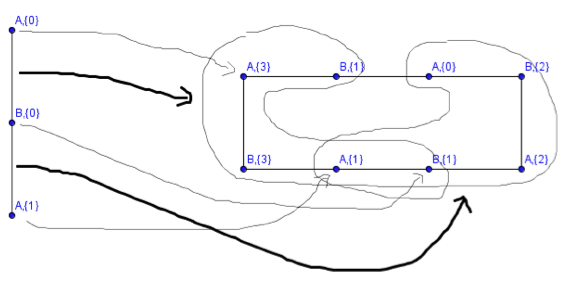
\includegraphics[scale=0.65]{Figura1.png}
    \end{center}

    \begin{enumerate}
      \item{Demuestra que existe un protocolo que puede resolver la tarea,
        considera que se puede ejecutar más de una lectura y escritura sobre
        el mismo arreglo mem[A,B]}
      \item{Demuestra que con un protocolo de una ronda no se puede resolver el 
          problema}
    \end{enumerate}
  }

\item{
    Sea $\delta$ un mapeo simplicial, que nos lleva de una gráfica $G$ a una
    gráfica $H$, $\delta$ mapea los vértices de $G$ sobre todos los vértices de
    $H$.
    \begin{enumerate}
      \item{Demuestra que si $G$, es conexo entonces $H$ es conexo.}
      \item{Demuestra que si $\delta$ preserva colores entonces es rigido, es
        decir, mapea vertices diferentes a vértices diferentes.}
    \end{enumerate}
  }

\item{
    Considera protocolos de una sola iteración de memoria compartida libre de
    espera, y un complejo de entrada $\mathcal{I}$ de N vértices y M aristas,
    define una tarea $\langle \mathcal{I},\mathcal{O},\Delta \rangle$, sobre
    este complejo que se pueda resolver, suponer que $\Delta (v)$ siempre es
    un sólo vértice, tal que
    \begin{enumerate}
      \item{el número de soluciones posibles (protocolos) sea lo mejor posible,
          y}
        \item{que sea lo mayor posible. En ambos casos, explica cual es ese
            número.}
    \end{enumerate}
  }

\item{
    Presenta una caracterización de las tareas que tienen solución mediante este
    tipo de protocolos, protocolos del ejercicio 3, y un algoritmo (secuencial)
    que tome como entrada una tarea, y como salida diga si tiene o no solución.
    ¿Cuál es la complejidad de tu algoritmo?
  }
\end{enumerate}
\end{document}